%!TEX root=./notes_template.tex

\noindent\textbf{Counting Involutions}

\begin{theorem}
    Let $I_n$ denote the set of involutions of $S_n$. Then $|I_n|$ is given by the following recurrence.
    \[
        |I_n|=\begin{cases}
            1 & n=1\\
            2 & n=2\\
            I_{n-1}+(n-1)I_{n-2} & n>2
        \end{cases}
    \]
\end{theorem}
\begin{proof}
    Note that $S_1$ only has the identity permutation and that $S_2$ consists of the identity permutation and the
    transposition $\sigma:=(2\; 1)$. Obviously $id^2=id$ and $\sigma^2=id$. Thus $|I_1|=1$ and $|I_2|=2$. Now let
    $\sigma\in I_n$ for $n>2$. We now consider two cases, if $\sigma(n)=n$ and if $\sigma(n)\neq n$. We first assume
    that $\sigma(n)=n$. Then the restriction of $\sigma$ to the set $\{1,2,\ldots,n-1\}$, $\widetilde{\sigma}$ has image
    $\{1,\ldots,n-1\}$ and thus $\widetilde{\sigma}$ is surjective onto $\{1,\ldots,n-1\}$. Ergo $\widetilde{\sigma}$
    can be viewed as an element of $S_{n-1}$. Moreover, note that $\sigma^2=id$ and thus, for all $i\in\{1,\ldots,n-1\}$,
    $\widetilde{\sigma}^2(i)=\sigma^2(i)=i$ and $\widetilde{\sigma}\in I_{n-1}$. Now suppose $\sigma(n)=j\neq n$. Then
    the restriction of $\sigma$ to the set $A:=\{1,\ldots,j-1\}\sqcup\{j+1,\ldots,n-1\}$, $\widehat{\sigma}$, has $A$ as
    its image. Again note that, by re-indexing, $\widehat{\sigma}$ can be viewed as an element of $S_{n-2}$ and that
    $\widehat{\sigma}^2=id$. Thus $\widehat{\sigma}\in I_{n-2}$.

    On the other hand, any involution in $S_{n-1}$ can be extended to an involution in $S_n$ by sending $n\mapsto n$
    and any involution of $\{1,\ldots,j-1\}\sqcup\{j+1,\ldots,n-1\}$ can be extended to an involution in $S_n$ by
    sending $j\mapsto n$ and $n\mapsto j$. It is easy to see that these restriction and extension operations are mutually
    inverse maps between $I_n$ and $I_{n-1}\sqcup\bigsqcup_{j=1}^{n-1} I(\{1,\ldots,j-1\}\sqcup\{j+1,\ldots,n-1\})$ where
    $I(A)$ is the set of involutions on a set $A$. This yields that, for $n>2$,
    \[
        |I_n|=|I_{n-1}|+\sum_{j=1}^{n-1}|I(\{1,\ldots,j-1\}\sqcup\{j+1,\ldots,n-1\})|=|I_{n-1}|+(n-1)|I_{n-2}|
    \] 
    via re-indexing.
\end{proof}

\noindent\textbf{Inversions}

\begin{definition}
    Let $\sigma\in S_n$. Then the pair $(i,j)$ where $1\leq i< j\leq n$ is an \textit{inversion pair} if
    $\sigma(i)>\sigma(j)$.
\end{definition}

\begin{example}
    Let
    \[
        \sigma = \begin{pmatrix}
            1&2&3&4&5&6&7\\
            6&5&1&2&7&4&3
        \end{pmatrix}
    \]
    then the inversion pairs of $\sigma$ are
    \[
        \begin{array}{lllll}
            (1,2),&(1,3),&(1,4),&(1,6),&(1,7)\\
            (2,3),&(2,4),&(2,6),&(2,7)\\
            (5,6),&(5,7)\\
            (6,7)
        \end{array}
    \]
\end{example}

\begin{definition}
    Let $\sigma\in S_n$. Then the \textit{length} of $\sigma$, denoted $l(\sigma)$, is the number of inversion pairs of
    $\sigma$. Moreover, we say that $\sigma$ is \textit{odd} if $l(\sigma)$ is odd and \textit{even} if $l(\sigma)$ is
    even. The \textit{signature} of $\sigma$ is $\text{sign}(\sigma)=(-1)^{l(\sigma)}$.
\end{definition}

\noindent\textit{Question:} What is the maximum number of inversions an element of $S_n$ can have?

\noindent Since we have one inversion per pair of elements out of order, we can maximize the number of inversions by
making it so that \textit{every} pair is out of order. In particular, we do this by writing the elements of
$\{1,\ldots,n\}$ in descending order. The permutation that does this is $\sigma=(n\;n-1\;\ldots\;1)$. We can then count
the number of inversions to get that $\sigma$ has $(n-1)+(n-2)+\ldots+1=\binom{n}{2}$ inversions. Thus the maximum
number of inversions of an element in $S_n$ is $\binom{n}{2}$.

\begin{definition}
    The \textit{alternating group} is the (normal) subgroup of $S_n$ containing all even permutations of $S_n$.
\end{definition}

\begin{example}
    \[
        \begin{array}{rrccccccl}
            S_3=&\{&e,&(1\;2\;3),&(2\;1\;3),&(2\;3\;1),&(3\;1\;2),&(3\;2\;1)&\}\\
            l(\sigma)=&&0&1&1&2&2&3
        \end{array}
    \]
    This tells us that $A_3=\{e,(2\;3\;1),(3\;1\;2)\}$.
\end{example}

\begin{theorem}
    If $n\geq 2$, then $|A_n|=\frac{n!}{2}$.
\end{theorem}
\begin{proof}
    For convenience we will say that $S_n$ is the group of permutations on $\{0,1,\ldots,n-1\}$.
    Note that length is a map $l:S_n\to\ZZ$ Thus we can write $S_n=l^{-1}(2\ZZ)\sqcup l^{-1}(2\ZZ+1)$ that is
    we can write $S_n$ as the disjoint union of $A_n$ and the odd permutations $O_n$. Thus, $n!=|S_n|=|A_n|+|O_n|$.
    Let $\phi:S_n\to S_n$ be given by $\phi(\sigma)=\sigma\circ(1\;0)$. Since $\phi$ is given by precomposition with an
    involution, we get that $\phi^2=id$. We now claim that $l(\phi(\sigma))=l(\sigma)\pm 1$. Now consider $\phi(\sigma)$.
    \[
        \phi(\sigma)=
        \begin{pmatrix}
            0&1&2&\ldots&n-1\\
            \sigma_0&\sigma_2&\sigma_3&\ldots&\sigma_n
        \end{pmatrix}
        \begin{pmatrix}
            0&1&2&\ldots&n-1\\
            1&0&2&\ldots&n-1
        \end{pmatrix}
        =
        \begin{pmatrix}
            0&1&2&\ldots&n-1\\
            \sigma_1&\sigma_0&\sigma_2&\ldots&\sigma_{n-1}
        \end{pmatrix}
    \]
    Now consider any inversion pair $(i,j)$ of $\sigma$.
    If $i,j\geq 2$, then by inspecting the above formula, we see that $(i,j)$ is an inversion pair of $\sigma$ iff $(i,j)$
    is an inversion pair of $\phi(\sigma)$. Additionally, if $i=0,1$ and $j\geq2$, then $(i,j)$ is an inversion pair of
    $\sigma$ iff $(i+1\mod 2,j)$ is an inversion pair of $\phi(\sigma)$. Moreover, $(0,1)$ is an inversion pair of $\sigma$
    iff $(0,1)$ is \textit{not} an inversion pair of $\phi(\sigma)$. Thus $\phi(\sigma)$ either has one more or one fewer
    inversion pair than $\sigma$ as desired. Thus we can write $\widetilde{\phi}=\phi|_{A_n}:A_n\to O_n$ and
    $\widehat{\phi}=\phi|_{O_n}:O_n\to A_n$. Additionally,
    $\widetilde{\phi}\circ\widehat{\phi}=id_{O_n}$ $\widehat{\phi}\circ\widetilde{\phi}=id_{A_n}$ since $\phi^2=id_{S_n}$.
    Thus $\widetilde{\phi}$ is a bijection and $|A_n|=|O_n|$. Ergo, $n!=2|A_n|$ as desired.
\end{proof}

\noindent\textbf{Graphical Depictions for Permutations}

\begin{definition}
    Each $\sigma\in S_n$ corresponds uniquely to its \textit{Rothe Diagram}, an $n\times n$ grid with a $\cdot$ in column
    $i$, row $\sigma_i$ where every square to the right of a dot and every square below a dot is blotted out.
\end{definition}

\begin{example}
    Here is the Rothe diagram for $(6\;7\;1\;4\;2\;3\;5)$

    \begin{figure}[h]
        \centering
        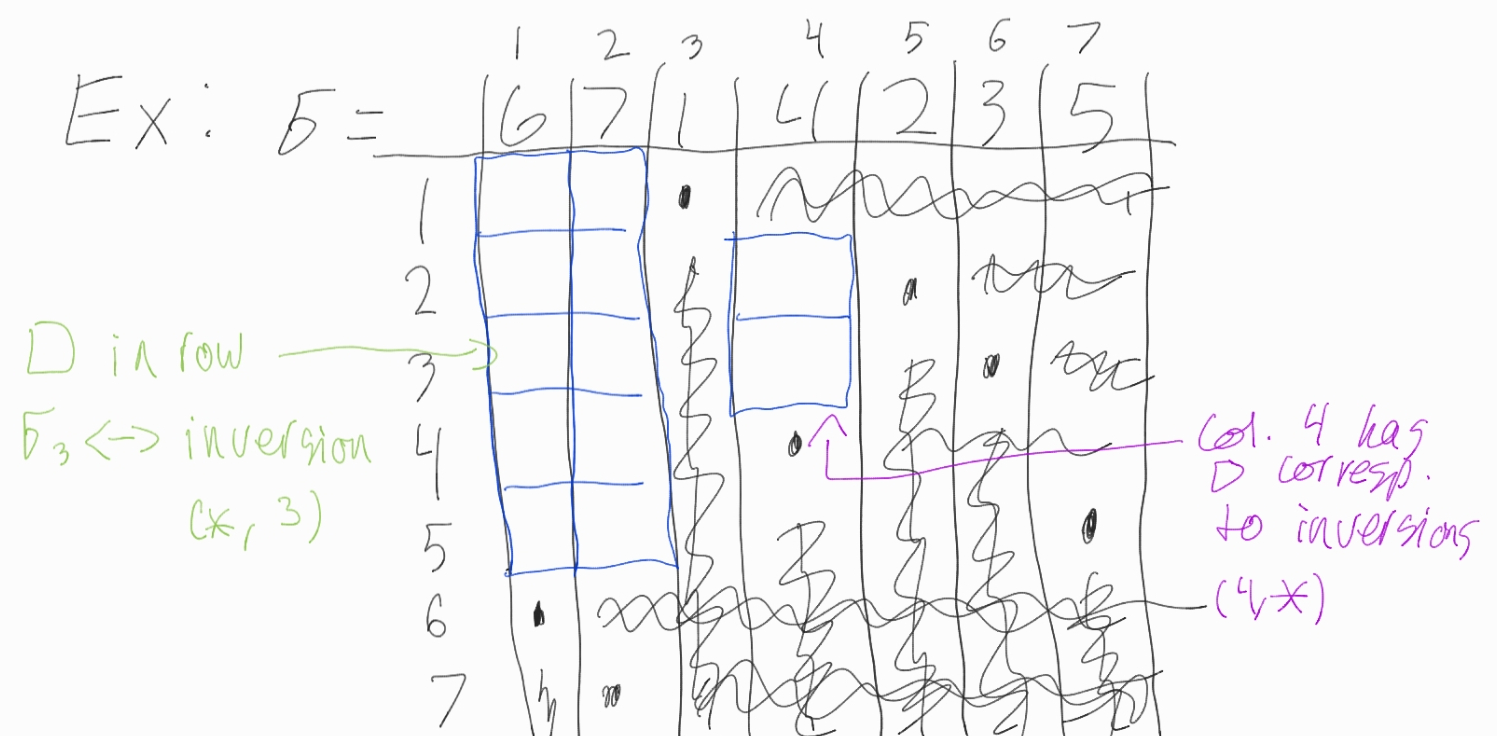
\includegraphics[scale=0.28]{images/rothe-diagram-1.jpg}
    \end{figure}

\end{example}

\noindent Note that the dots form a permutation matrix for the permutation.

\noindent\textit{Question:} What are the inversions of $(6\;7\;1\;4\;2\;3\;5)$?

\[
    (1,3),(1,4),(1,5),(1,6),(1,7),(2,3),(2,4),(2,5),(2,6),(2,7),(4,5),(4,6)
\]

\noindent However, we can figure these out from the Rothe diagram!

\begin{theorem}
    For any $\sigma\in S_n$, there is an unblotted square in column $i$ row $\sigma_j$ of the Rothe diagram
    iff $(i,j)$ is an inversion pair.
\end{theorem}

\begin{proof}
    \textbf{TODO}
\end{proof}

\begin{corollary}
    The number of blank squares in column $i$ of a Rothe diagram is the number $j>i$ such that $\sigma_i>\sigma_j$,
    that is the number of $j$ such that $(i,j)$ is a inversion pair.
\end{corollary}

\noindent\textbf{Lehmer Codes}

\begin{definition}
    The Lehmer code of a $\sigma\in S_n$ is $c(\sigma)=(c_1,c_2,\ldots,c_{n-1})$ where $c_i$ is the number of $j$ such
    that $\sigma_i>\sigma_j$, that is $c_i$ is the number of $j$ such that $(i,j)$ is an inversion pair.
\end{definition}

\noindent Note that $c(\sigma)$ is a vector of length $n-1$ since the last entry in a permutation cannot form an
inversion pair with it as the first entry.

\begin{example}
    For $\sigma=(6\;7\;1\;4\;2\;3\;5)$, $c(\sigma)=(5,5,0,2,0,0)$.
\end{example}

\begin{theorem}
    The Lehmer code is a bijection between $S_n$ and $L_n=\{(v_1,\ldots,v_{n-1})\in\ZZ^{n-1}|0\leq v_i\leq n-i\}$.
\end{theorem}

Note that by a quick count, we see that $|L_n|=n!=|S_n|$. Thus in order to prove that the Lehmer code is a bijection, it
suffices to show that for any $v\in L_n$, there exists a $\sigma\in S_n$ such that $c(\sigma)=v$.

\begin{lemma}
    Let $v=(v_1,\ldots,v_{n-1})\in L_n$, then the following procedure constructs a Rothe diagram whose corresponding
    permutation, $\sigma$, has $c(\sigma)=v$.
    \begin{algorithmic}
        \State Let $D$ be an empty $n\times n$ grid.
        \ForAll{$i\in\{1,2,\ldots,n-1\}$}
            \State Place a $\cdot$ in column $i$ such that there are $v_i$ blank squares above it.
            \State Blot out all cells below this dot and blot out all cells to the right of this dot.
        \EndFor
        \State Fill in the only remaining cell in column $n$.
    \end{algorithmic}
\end{lemma}

\begin{proof}
    In order to prove this lemma, we must show the following.
    \begin{enumerate}
        \item The algorithm terminates.
        \item The algorithm can proceed at each step. That is, there is always a space in which we can place our dot so
        that there are $v_i$ blank squares above it.
        \item The output diagram is a Rothe diagram.
        \item The corresponding permutation has Lehmer code $v$.
    \end{enumerate}

    The details are \textbf{TODO}.
\end{proof}

\bigskip

\section*{\bf Homework 2}



\begin{enumerate}
    \item Draw the Rothe diagram for the permutation $(2\; 5\; 7\; 4\; 6\; 1\; 3)$.
    \item Implement the algorithm described in the above lemma in Python/Sage. No cheating using built-in Sage commands!
    Make sure to test it with some examples (like the one from number 1).
\end{enumerate}
